\chapter{State of the art} % Main chapter title

%-------------------------------------------------------------------------------
%---------
%
\section{Research Questions}

For the literature review and stat of the art analysis, two research questions have been formulated to address the essential background and focus of this dissertation. The first research question centers on the fault tolerance mechanisms of each language under study. The second research question examines the benchmarking strategies that simulate distributed systems, such as microservices, and identifies the metrics necessary for accurately measuring each case.

\begin{itemize}
    \item \textbf{RQ1:} How do the programming languages Elixir, Scala with Akka, and Go implement fault tolerance mechanisms in distributed systems, and what are the comparative strengths, weaknesses, and trade-offs of each approach?
    \item \textbf{RQ2:} What are the most effective benchmarking strategies for simulating distributed environments, and which metrics are most relevant for evaluating fault tolerance in these scenarios?
\end{itemize}

\subsection{Research Methodology}

This section outlines the research methodology adopted in this dissertation. It is important to note that this study addresses a gap in the literature regarding a direct comparison of fault tolerance mechanisms in the programming languages Elixir, Scala with Akka, and Go. To the best of our knowledge, no prior study has evaluated these three languages side-by-side in fault-tolerance test scenarios. 

However, relevant groundwork can be found in the study by Valkov et al. \cite{Valkov2018}, which compared Erlang, Go, and Scala in terms of inter-process communication latency, process creation time, the maximum number of supported processes, and throughput. This work serves as a valuable reference, but it does not delve into fault-tolerance aspects, which this dissertation seeks to address.

To explore the existing body of knowledge and identify studies relevant to the three programming languages, searches were conducted in major academic databases, specifically IEEE Xplore and ACM Digital Library. The objective was to find articles that included the three languages in their titles, allowing for Erlang to be considered in place of Elixir. The search was initiated with a starting date of 2013, coinciding with the publication of the second edition of Joe Armstrong's book on Erlang. However, the search yielded no results in the IEEE Xplore database, while the ACM Digital Library returned only two articles, ultimately filtering down to the work by Valkov et al.

\textbf{IEEE Xplore Query:}
\begin{verbatim}
"query": { 
    ("Document Title": "Elixir" OR "Document Title": "Erlang") AND
    ("Document Title": "Go" OR "Document Title": "Golang") AND 
    ("Document Title": "Akka" OR "Document Title": "Scala") 
}
\end{verbatim}



\textbf{ACM Digital Library Query:}
\begin{verbatim}
"query": { 
    Title:((Elixir OR Erlang) AND (Go OR Golang)) 
}
"filter": {
     E-Publication Date: (01/01/2013 TO 12/31/2024), ACM Content: DL 
}
\end{verbatim}


\textbf{RQ1: How do the programming languages Elixir, Scala with Akka, and Go implement fault tolerance mechanisms in distributed systems, and what are the comparative
strengths, weaknesses, and trade-offs of each approach?} 

Given the scope of the research question, developing a research strategy that yields precise and relevant results it challenging. Fault tolerance is a broad subject, spanning diverse areas from hardware to electronic devices until critical systems. Moreover, the programming languages under study are employed in varied contexts, such as Elixir’s popularity in \gls{IoT} and Go’s extensive use in microservices, at the same time being general purpose languages used in diverse areas. This diversity introduces complexity when conducting research queries, resulting in an huge volume of information on a wide range of topics, or the lack of results in a more narrow query like the following one:

\begin{verbatim}
"query": { 
    Abstract:(
        ("fault tolerance" OR "error handling" OR "resilience") AND
        ("distributed systems" OR "microservices" OR "software") AND 
        ("Elixir" OR "Scala" OR "Akka" OR "Go" OR "Golang" OR "Erlang")
    )
}
\end{verbatim}

To address this, the methodology employed covered grey literature, particularly books, due to their mature, structured content. Books provide comprehensive insights into foundational principles, and given that the evolution of programming languages tends to be gradual, they serve as reliable resources for understanding their core concepts and implementations, taking in consideration the choose of recently books. At the same time, white literature, including academic papers and recent articles, was included to capture the latest advancements, structures, and innovations within these languages. 

Given the technical and practical focus of the study, a more ad-hoc research approach was adopted, like searching on the academic databases for more focused themes, not systematic queries or keywords. Official documentation for each language it was also consulted, as it provides up-to-date information directly from the creators. Furthermore, trusted blogs and community resources were consulted in order to utilize the collective knowledge and practical experiences of developers, which often provide valuable insight that may not be addressed elsewhere. 

\textbf{RQ2: What are the most effective benchmarking strategies for simulating distributed environments, and which metrics are most relevant for evaluating fault tolerance in these scenarios?}

...

\section{Elixir Programming Language Analysis}

The following sections provide an overview of Elixir and its foundational principles within the Erlang ecosystem. This discussion will explore how the ecosystem relates to Elixir's modernization and how it enhances fault tolerance. Additionally, the fault tolerance strategies employed within this ecosystem will be examined, including their drawbacks and real-world applications.

\subsection{The Foundation of Erlang}

Elixir is built on top of Erlang, making it essential to first understand Erlang’s core principles and environment to move into Elixir’s capabilities. Elixir leverages Erlang’s foundation for constructing fault-tolerant and distributed systems, benefiting from its mature ecosystem and proven reliability \cite{Juric2024,Armstrong2013}.

Erlang, developed in the mids of 1980s by Ericsson, was specifically designed to support systems that are highly reliable, responsive, scalable, and always available \cite{Armstrong2013,Juric2024}. Over the years, Erlang has evolved significantly, and Elixir represents a major milestone in this environment's evolution. Elixir enhances the ecosystem with modern features, such as a more developer-friendly syntax, powerful metaprogramming capabilities with macros, and improved tooling, all while maintaining full compatibility with the Erlang runtime \cite{Juric2024}. This success is closely tied to its coupling with Erlang’s semantics, also the inclusion of the \gls{OTP}, which provides robust libraries and tools. Additionally, Elixir inherits the power of \gls{BEAM}, the Erlang \gls{VM}, which could be considered as a state of art concurrent programming model \cite{erlang-concurrency-blog}.

\subsubsection{Concurrency in Erlang and BEAM}

Concurrency is one of the most defining aspects of the Erlang environment, earning it the title of being a concurrency oriented language by many. At the heart of this model are processes, which adhere to the Actor Model \cite{Juric2024,Valkov2018}. In this paradigm, each process acts as an independent actor, being lightweight and isolated, communicating with others through message-passing via mailboxes. These processes differ from heavyweight \gls{OS} processes or threads, which rely heavily on the operating system for management and lack the flexibility needed for fine-grained optimization. For instance, in the \gls{JVM}, platform threads are a thin abstraction over \gls{OS} threads, limiting control and optimization. However, virtual threads, introduced on Java 21, brings more capabilities to the \gls{JVM}, where the Akka framework take advantage of \cite{erlang-concurrency-blog}.

In contrast, \gls{BEAM} employs a concurrency-oriented programming model in which one thread per \gls{CPU} core manages numerous lightweight processes. This architecture enables \gls{BEAM} to handle parallelism by letting one scheduler per \gls{CPU} handling multiple lightweight processes. This strategy is illustrated in Figure \ref{fig:beam-process}, where this architecture enables fault tolerance aspects over isolating the processes \cite{Juric2024}.

\begin{figure}
    \centering
    \frame{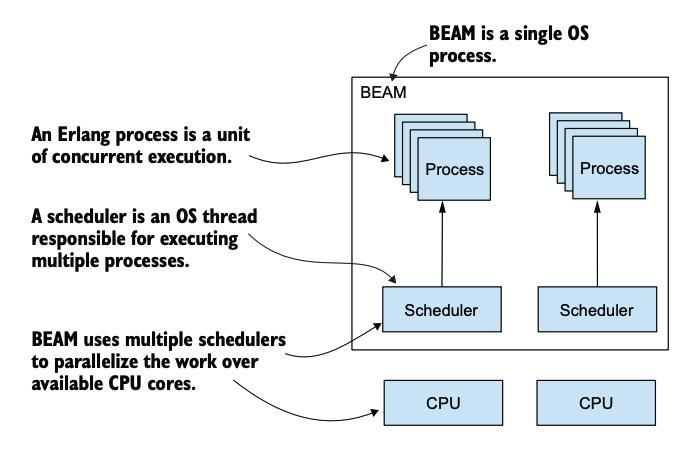
\includegraphics[width=120mm]{ch-state/assets/beam-process.png}}
    \caption[Concurrency in the Erlang virtual machine]{Concurrency in the Erlang virtual machine. Adapted from \cite{Juric2024}.}
    \label{fig:beam-process}
\end{figure}

The \gls{BEAM} scheduler is considered preemptive, meaning that assigns short execution time slices to each process. This ensures that long-running tasks do not monopolize system resources, promoting fairness and responsiveness \cite{Armstrong2013}. Also, it promotes fault tolerance characteristic by stopping processes carried with permanent faults, where on a non-preemptive scheduler could harm the overall system. Processes that are blocked due to I/O operations or waiting for messages are efficiently managed by separate threads or a kernel polling service, preventing unnecessary CPU usage and ensuring that waiting processes do not hinder the execution of others \cite{Juric2024,erlang-concurrency-blog}.

\begin{figure}
    \centering
    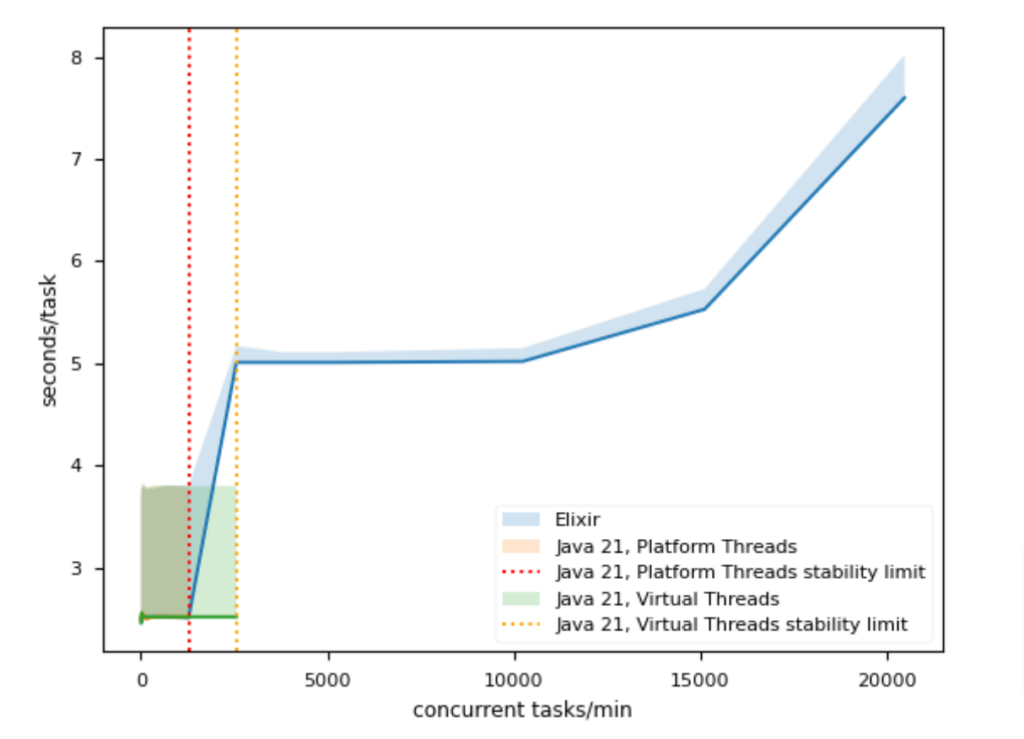
\includegraphics[width=120mm]{ch-state/assets/elixir-vs-jvm-threads}
    \caption[Elixir/BEAM processes vs JVM threads]{Elixir/BEAM processes vs JVM threads. Adapted from \cite{erlang-concurrency-blog}.}
    \label{fig:beam-vs-jvm}
\end{figure}

In a direct comparison of Elixir’s processes running on \gls{BEAM} with the two threading techniques of the \gls{JVM}, as illustrated in Figure \ref{fig:beam-vs-jvm}, notable differences appears. Under low load conditions, all three strategies, Elixir’s lightweight processes, the \gls{JVM}’s platform, and virtual threads, perform effectively. However, as the system approaches the stability limits of platform threads, approximately 2500 threads, Elixir continues to handle additional processes, scaling up to approximately 200,000 concurrent processes. Although the per-task completion time increases slightly under such high loads, the system remains operational and stable. The opposite occurs with both \gls{JVM} techniques, resulting in an overload that makes maintaining pace impossible. Furthermore, \gls{BEAM} imposes a theoretical limit of roughly 134 millions processes, where this limit are lowered where the underlying implementation are a direct relationship with \gls{OS} threads \cite{Juric2024}.

This scalability advantage can be attributed to the architecture of the underlying \gls{BEAM}. Unlike the \gls{JVM}, which relies on a shared heap and tightly integrates with \gls{OS} threads. However, the \gls{JVM} threading model is better suited for low-concurrency scenarios involving long-lived threads. In contrast, Elixir/\gls{BEAM} excels in high-concurrency situations with short-lived processes \cite{erlang-concurrency-blog, Valkov2018}.

\subsubsection{Garbage Collection and Immutability}

Erlang and Elixir enforce immutability as a fundamental principle, ensuring that all data remains unchangeable. This eliminates many concurrency issues common in systems with shared memory, such as race conditions. Instead of sharing memory, processes communicate by passing immutable data. When a message is sent, the receiving process creates a copy of the data in its stack, eliminating the need for semaphore controls or similar synchronization mechanisms \cite{Juric2024,erlang-concurrency-blog}.

Because processes are completely isolated and do not share memory, \gls{BEAM} can execute garbage collection at the process level. This per-process garbage collection allows the \gls{VM} to reclaim memory for a single process without pausing the entire system, unlike the global garbage collection approach commonly used in the \gls{JVM}, where all processes share a single heap. Additionally, \gls{BEAM} optimizes garbage collection by focusing on individual schedulers enhancing its efficiency \cite{Armstrong2013,Juric2024}.

The garbage collector can significantly impact the performance of both the \gls{BEAM} and \gls{JVM}. As illustrated in Figure \ref{fig:beam-vs-jvm}, the load on \gls{BEAM} outperforms that of the \gls{JVM}. This difference may be attributed to the \gls{JVM}'s "stop-the-world" garbage collection, which can create performance bottlenecks. In contrast, \gls{BEAM} utilizes a more targeted garbage collection approach, benefiting from process isolation, which can lead to enhanced performance \cite{Valkov2018, Juric2024}.

\subsubsection{Hot-code swapping}

Hot-code swapping is a beneficial feature for building fault-tolerant systems, allowing the modification of code that is actively running in real time. This mechanism enhances fault tolerance by enabling the replacement of fault code without requiring system downtime. The process is typically achieved by sending a message to the server, which then handles the exchange \cite{Armstrong2013}.

It is important to note that this capability is not implemented in the same way on the \gls{JVM}. While the \gls{JVM} supports class reloading, it is not comparable to hot-code swapping of \gls{BEAM} and introduces significant complexities, such as managing already instantiated objects. In contrast, the hot-code swapping mechanism in systems that rely on \gls{BEAM} allow targeted changes, focused on specific parts without disrupting the system \cite{erlang-concurrency-blog}. Furthermore, in comparison with the Go language, which is a compiled language, does not permit hot code swapping in a production environment natively \cite{go-docs}.

\subsection{Fault Tolerance Mechanism and Strategies}

Elixir's fault tolerance strategies and mechanisms are associated to the Erlang ecosystem, leveraging the features of the \gls{BEAM}. A fundamental aspect of Elixir's fault tolerance is its adherence to the "let it crash" philosophy, which, combined with the actor model and extensive support from third-party tools, enhances its resilience. This is elaborated upon in the following sections.

\subsubsection{Let It Crash Philosophy and Actor Model}

Elixir inherits the “let it crash” philosophy from Erlang, which forms the foundation of its fault tolerance strategy. This philosophy is based on the principle that failures are unavoidable in distributed systems, and the optimal approach is not to prevent them entirely but to design systems that can recover autonomously and gracefully \cite{Armstrong2013, Kleppmann2017}. Instead of defensive programming to anticipate every potential error, Elixir encourages developers to isolate processes so that faults can occur without compromise the stability of the entire system \cite{Juric2024}.

The Actor Model plays a central role in achieving this resilience. In Elixir, lightweight processes act as independent actors that do not share memory and communicate exclusively through message-passing. When a process encounters an unrecoverable error, it is allowed to fail and terminate. This termination is both deliberate and beneficial, as it enables easy fault detection and ensures that failures do not propagate, preserving the integrity of the overall system \cite{Juric2024,Armstrong2013}. This model naturally integrates with the Supervisor pattern, which is one of Elixir’s primary mechanisms for fault recovery.

\textit{\underline{Supervisor Pattern}}

The Supervisor pattern is a practical implementation of the “let it crash” philosophy, built on the Actor Model. While the concept is not exclusive to Elixir, other frameworks like Akka also use it, Elixir leverages this pattern to build fault-tolerant systems \cite{Valkov2018}. In this approach, processes are classified into two types \cite{Juric2024}:

\begin{itemize}
    \item \textbf{Workers:} Processes that perform tasks or contain application logic but do not oversee other processes.
    \item \textbf{Supervisors:} Processes responsible for monitoring and managing other processes.
\end{itemize}

\begin{figure}
    \centering
    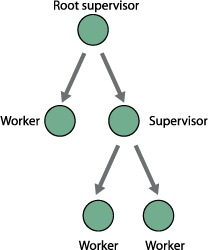
\includegraphics[scale=0.7]{ch-state/assets/supervisor-design.jpg}
    \caption[Supervisor tree pattern]{Supervisor tree pattern. Adapted from \cite{Juric2024}.}
    \label{fig:supervisor-pattern}
\end{figure}

Supervisors are organized into a hierarchical supervision tree, as illustrated in Figure \ref{fig:supervisor-pattern}. This tree defines the relationships between supervisors and workers, with each supervisor managing a group of processes. This structure provides modularity and ensures that fault recovery is localized, reducing the impact of failures \cite{Armstrong2013}.

Supervisors in Elixir operate using restart strategies to determine how to handle failures. The options given by the \gls{OTP} Supervisors and the most common ones are the following \cite{elixir-docs-hexdocs,Juric2024,Armstrong2013}:
\begin{itemize}
    \item \textbf{One-for-One:} If a single worker process fails, the supervisor restarts only that process.
    \item \textbf{One-for-All:} If one process fails, the supervisor restarts all processes it manages.
    \item \textbf{Rest-for-One:} If a process fails, the supervisor restarts it and all other processes started after it in the hierarchy.
\end{itemize}

Each restart strategy addresses specific use cases. Additionally, supervisors can enforce restrictions on the restart process through a restart frequency configuration. This mechanism monitors the frequency of the worker process failures within a specified time frame. If a worker process fails repeatedly and exceeds the configured threshold, the supervisor itself terminates to avoid harming the system or entering an infinite restart loop \cite{Armstrong2013}.

The One-for-One strategy is best suited for independent processes \cite{Armstrong2013}. For instance, in a web server handling multiple concurrent requests, this strategy could allow for the rapid recovery of a single failed process without affecting others. In contrast, the One-for-All strategy is ideal for tightly coupled processes \cite{Armstrong2013}. When one process fails, all other processes under the same supervisor are restarted, this could be useful for processes that need synchronization among them. Finally, the Rest-for-One strategy could be used in workflows with sequential dependencies \cite{elixir-docs-hexdocs}. For example, in a data pipeline where each stage relies on the output of the previous stage, a failure in one process triggers the restart of the failed process along with any subsequent ones.

The supervision pattern is not uniquely associated with Elixir, it is also used in other languages that follow the Actor Model, as well as in various frameworks that implement this programming style. One of the most notable \gls{JVM} frameworks is Akka. Additionally, in other paradigms such as Go, there are libraries capable of unifying \gls{CSP} with the Actor Model, such as the proto.actor library.


\subsubsection{Tools and Support}

Elixir’s state of art in the fault tolerance area is related to the integration with the Erlang ecosystem, the \gls{BEAM}, the Actor Model, and the “let it crash” philosophy. These elements are further enhanced by Elixir’s compatibility with the \gls{OTP}, which provides a suite of design principles and tools for building fault-tolerant and distributed systems. This integration allows Elixir inherit and extend the mechanisms that have been tested and proven in real case scenarios \cite{Juric2024,Armstrong2013}.

The \gls{OTP} framework enables Elixir to use the Supervision Tree pattern, an important element on fault tolerance like described early. By combining the Supervision Tree with tools like GenServer, Elixir simplifies the management of stateful processes, facilitates concurrent operations, and ensures the efficient handling of asynchronous message passing \cite{elixir-docs-hexdocs}.

Additionally, \gls{OTP} supports features like hot-code swapping, enabling systems to update running code in real-time without downtime. The inclusion of the Mnesia distributed database within \gls{OTP} further strengthens Elixir’s fault tolerance capabilities. Mnesia allows state storage across distributed nodes, ensuring data consistency and availability even in the presence of node failures \cite{elixir-docs-hexdocs,elixir-school}.

Beyond the core features of \gls{OTP}, Elixir also includes Mix, a build tool that simplifies dependency management, testing, project configuration, and documentation generation. Mix integrates into the Elixir ecosystem, streamlining development workflows and contributing to the reliability of applications by ensuring consistent builds\cite{elixir-docs-hexdocs,elixir-school}.

In addition to the built-in capabilities of \gls{OTP}, Elixir’s ecosystem benefits from third-party projects that extend its fault-tolerant capabilities. For instance, Graft, developed by Le Brun et al. \cite{LeBrun2021} in 2019, and Ra, developed by the RabbitMq team 
\footnote{Ra: \url{https://github.com/rabbitmq/ra/} (accessed 4 December 2024)}
, provide an implementation of the Raft consensus algorithm. Similarly, the Fuse library
\footnote{Fuse: \url{https://github.com/jlouis/fuse/} (accessed 4 December 2024)}, 
a widely-used implementation of the Circuit Breaker pattern, developed in Erlang, is also compatible with Elixir.

Another aspect of Elixir that is important to reference is its metaprogramming capabilities through macros, which allow developers to write code that generates code. This enables the Elixir codebase to be partially constructed using its own macros, extending the language's functionality and reducing boilerplate \cite{Juric2024}.

Lastly, it's important to mention the Elixir environment, which includes frameworks that enhance software development. Phoenix
\footnote{Phoenix: \url{https://phoenixframework.org/} (accessed 4 December 2024)}
is a popular framework for building scalable web applications. It inherits Elixir's fault tolerance, allowing applications to handle errors gracefully and maintain uptime. Phoenix also supports real-time features through channels for live updates \cite{Juric2024}. Nerves
\footnote{Nerves: \url{https://nerves-project.org/} (accessed 4 December 2024)}
focuses on embedded systems, leveraging Elixir's fault tolerance to create resilient IoT devices. It simplifies firmware development and management, ensuring efficient hardware and system updates.

These integrations, extensions  demonstrate Elixir’s ability to not only leverage the proven robustness of \gls{OTP} but also adapt and grow through innovative tools and libraries, solidifying its position as a leading choice for building fault-tolerant, distributed applications. 

\subsubsection{Drawbacks and Real Applications}

The benefits of Elixir are closely tied to the powerful features of the \gls{BEAM}, as mentioned earlier. However, there are some drawbacks to consider. One major limitation is the lack of third-party libraries, despite \gls{OTP} providing good support. Currently, it is challenging for Elixir to compete with more popular languages in this regard. Additionally, although the \gls{BEAM} has a distributed nature, its single-threaded architecture with a garbage collector makes it less suitable for fault-tolerant applications in critical systems that require fault tolerance at low level \cite{Juric2024}.Another potential drawback of Elixir is that it is a dynamically-typed programming language, which can result in errors from type mismatches or programming mistakes \cite{Cassola2020}. In contrast, languages such as Scala, Java, and Go offer advantages in this regard due to their static typing. However, there have been efforts to introduce a type system to Elixir without sacrificing the language's inherent dynamism, as demonstrated in the work of Cassola et al. \cite{Cassola2020}.

Despite these limitations, Elixir has been successfully utilized in numerous prominent projects. Taking as reference the official website of Elixir, for example, Discord relies on Elixir as the backbone of its chat infrastructure, leveraging its ability to handle real-time communication effectively. PepsiCo also employs Elixir in a central role within its data pipeline, providing marketing and sales teams with tools to query, analyze, and integrate data from various search marketing partners. Other notable examples of Elixir's application include Heroku, SparkMeter, and several others.


\section{Scala Programming Language with Akka Toolkit Analysis}

\section{Go Programming Language Analysis}


\section{Benchmarking Strategies}


\section{Conclusions}